% Created 2022-05-05 Čt 20:18
% Intended LaTeX compiler: pdflatex
\documentclass[11pt]{article}
\usepackage[utf8]{inputenc}
\usepackage[T1]{fontenc}
\usepackage{graphicx}
\usepackage{longtable}
\usepackage{wrapfig}
\usepackage{rotating}
\usepackage[normalem]{ulem}
\usepackage{amsmath}
\usepackage{amssymb}
\usepackage{capt-of}
\usepackage{hyperref}
\author{Andrej Zaujec}
\date{\today}
\title{BDA Project: Platform for monitoring the nodes in ZCASH P2P network.}
\hypersetup{
 pdfauthor={Andrej Zaujec},
 pdftitle={BDA Project: Platform for monitoring the nodes in ZCASH P2P network.},
 pdfkeywords={},
 pdfsubject={},
 pdfcreator={Emacs 28.0.50 (Org mode 9.6)}, 
 pdflang={English}}
\begin{document}

\maketitle
\tableofcontents



\section{Introduction}
\label{sec:orgae2b13f}
The aim of this project is to monitor nodes in the Zcash P2P network. The monitoring of nodes should include the collection of metadata about nodes. The metadata consists of supported services, version and user-agent of node.
\section{Zcash protocol}
\label{sec:orge263eb7}
Nodes in the P2P are exchanging the information given the full compliance of protocol.
Zcash P2P protocol is based on the Bitcoin one and there is almost no difference in terms of encoding, headers and payload in these messages:
\begin{itemize}
\item version
\item verack
\item getaddr
\item addrv2
\end{itemize}
The session between two nodes starts with handshake.
The handshake is started with sending \texttt{version} message from one node and \texttt{verack} message sends as confirmation from other node. Then this process is repeated but the nodes are swapped. After this exchange of versions and confirmations, the session is established and further communication can follow. This means any node can ask the other one about transactions, peers or just ping him. With help of \texttt{getaddr} message and asking new nodes recursively, the P2P network can exposes almost all of the nodes participating.
The handshake process between clients looks like in \hyperref[fig-handshake]{Figure}.
\begin{figure}[htbp]
\centering
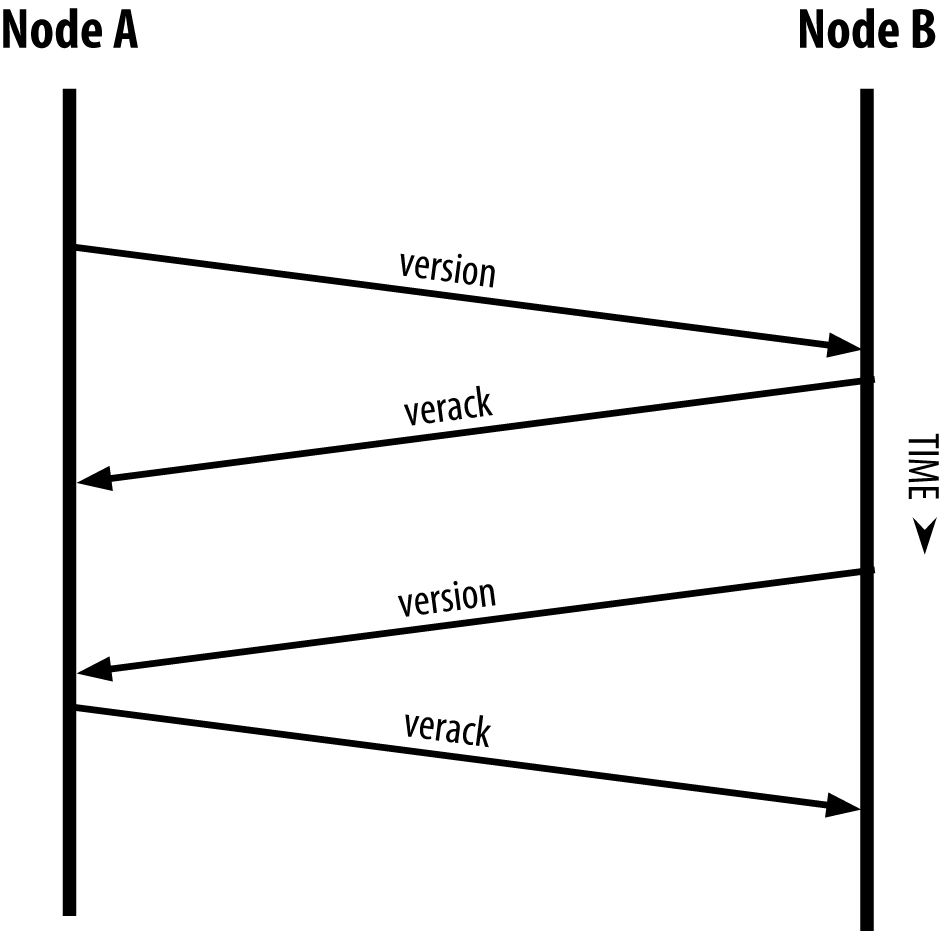
\includegraphics[width=.9\linewidth]{handshake.png}
\caption{\label{fig-handshake}Nodes handshake}
\end{figure}
The exact naming, data-types and values stored in protocol messages can be read in \href{https://developer.bitcoin.org/reference/p2p\_networking.html}{Bitcoin documentation}.
The most notice changes in the Zcash protocol are the magic bytes, protocol version numbering, default listening ports. Each mentioned change is described briefly below.
\begin{itemize}
\item magic bytes : Every message start with magic bytes, which are 4 hardcoded bytes that identifies the used network. The Zcash mainnet uses \texttt{24e92764} instead of Bitcoins \texttt{f9beb4d9}.
\item version numbering : The protocol version number shows what protocol version is client able to communicate in. Current Zcash nodes accepts only clients with version at least \texttt{170002} and higher. Bitcoin protocol version uses numbering from \texttt{70000}.
\item listening ports : The default port that Zcash client should listen on is \texttt{8233} port but the port can differ and it is not required from client to run only on this port.
\end{itemize}

\section{Design and implementation}
\label{sec:org92d3d81}
I do not like to reinvet the wheel so I did some analysis of similar projects and if they can be reused.
Firstly, I wanted to reuse the \href{https://github.com/fruit098/crypto\_monitor}{crypto monitor} project, which is monitoring platform for Bitcoin. The monitoring mechanism is based on the calling the bitcoin core client via RPC calls. The problem with Zcash client is that it does not have \texttt{getnodeaddresses} RPC call. This call exposes new node addresses from client, which is crucial feature in order for working. Without new addresses there will not be new peers and Zcash client does not have it as it was forked two years earlier from Bitcoin before adding the \texttt{getnodeaddresses} RPC call. So the approach with monitoring the network with help of Zcash official client and RPC calls is not suitable for this.

As I mentioned in Zcash protocol, the only difference between Zcash and Bitcoin in \texttt{version, verack, getaddr, addrv2} messages is the magic bytes constant and protocol version. This is perfectly suitable use-case for the \href{https://github.com/ayeowch/bitnodes/}{bitnodes} project, which already implemented the monitoring of nodes for Bitcoin. This solution is based on implemeting specific subset of protocol messages in order to look like of nodes but the implementation is interested only in creating new connections and obtaining possible new peer addresses. The problem with this solution is that is written in no more supported python 2 and the already mentioned differencies between Zcash and Bitcoin protocol.

This platform is based on the crawlig and protocol logic used from mentioned project bitnodes. The main improvements are rewriting it into python3, adding additional metadata and containerization of whole application. I did not made any major design changes to the crawlig and protocol logic used from bitnodes so I will describe how bitnodes does it as their project is
missing a whole documentation about main logic.

The application is based on the gevent coroutines, which enables utilizing multiple workers called greenlets to distribute the work. Thanks to the gevent greenlets the application is running in pseudo-parallel so it can be connected to the several thousands of nodes at the same time. Second major componenent is utilization of in-memory database called redis. The redis serves as the storage for the information about current connected, pending nodes. Each connected node has there metadata stored as well. The stored metadata are the user-agent, protocol version, IP, port, blockchain height, services. Brief description of crawling process and co-operation between workers and master will follow. The code is pretty self-explanatory so if there is some misunderstanding I recomend to read the code.
\subsection{Crawling}
\label{sec:orgb47e4c2}
Master greenlet will firstly make DNS resolution for the Zcash DNS seeds. The resolved IP addresses are added to the pending queue for the workers. Master will as well spawn all workers and start checking if the pending queue is not empty. Workers in the meantime are taking nodes information from the pending queue and trying to establish the connection with node. If the connection ends up succesfull, the worker will parse metadate about node and save the metadate under node specific key and put node IP and port under up queue to mark that this node is already connected. The worker will as well gather all the potentional node via \texttt{getaddr} and append them to pending queue. This same process process for workers is repeated until pending queue is exhausted when that happens master will dump and clear the up queue, which represents all connected nodes with metadata to the JSON and put every node from up queue to the pending queue to repeat whole process.





\section{Validation of results}
\label{sec:org2be1e02}
The described platform was run 38 times and each run it connected to then nodes ranging between 638 and 1600. On \hyperref[fig-platform]{Figure}, there are exact run times with the number of connected nodes that the platform connected to each run. The number of connections is listed as last in row. The interesting fact is that platform was able to crawl whole newtork under 4 minutes consistently with over 10000 connections attempt made per each run.
\begin{figure}[htbp]
\centering
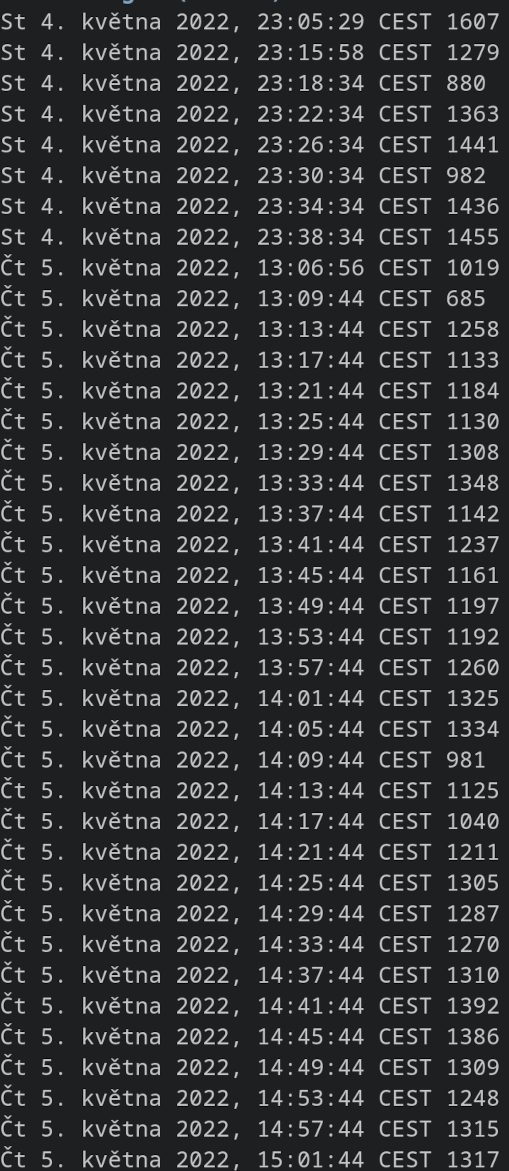
\includegraphics[width=200px]{platform_run.png}
\caption{\label{fig-platform}Platform run}
\end{figure}

On \hyperref[fig-output]{Figure}, there is example of JSON output, which is in form of array where the information from to bottom are IP, port, supported services, blockchain height, protocol version, user-agent.
\begin{figure}[htbp]
\centering
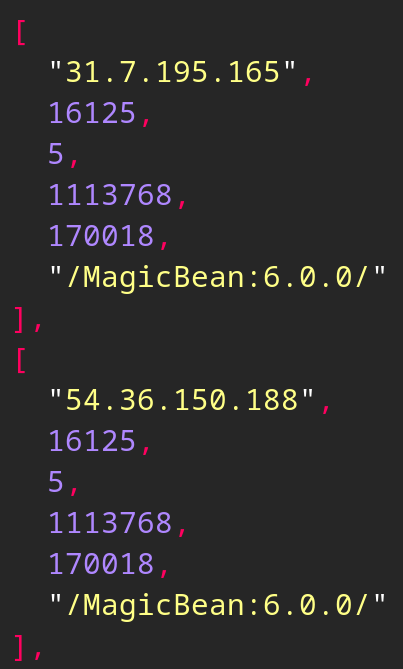
\includegraphics[width=200px]{output.png}
\caption{\label{fig-output}Example of JSON output}
\end{figure}



\section{Conclusion}
\label{sec:org3deff5b}
The implemented platform is able crawl whole Zcash P2P network under 4 minutes. This is thanks to the bitnodes low-level implementation of protocol, which makes communication much faster and focuses only on important part of creating new connectons with nodes and asking them for their peers. This fast execution is supported by python gevent coroutine package and in-memory database redis. Future improvement could be using the platform for other cryptocurrencies, which used the Bitcoin implementation as these currencies change protocol rarely. Other improvement could be implementing the ping mechanism from bitnodes in order to keep alive connection with connected node and monitor his activity regarding sending transactions or new peers.
\end{document}
